The \mf Storage (STO) Package simulates the contributions of specific storage and specific yield to the groundwater flow equations. Under confined conditions, in which the head above the top of the cell, storage changes are attributable solely to specific storage. Under unconfined conditions, in which the head is above the bottom but below the top of the cell, storage changes are attributable primarily to specific yield, but the contribution of specific storage is also taken into account.

In the original release of the \mf STO Package, the contribution of specific yield is formulated in terms of hydraulic head in a way that conserves water volume but renders the storage change under unconfined conditions dependent on the vertical datum relative to which heads and elevations are defined. Reexamination of the specific storage contribution in terms of pressure head leads to a revised formulation that eliminates the vertical datum dependence and still honors water conservation. This chapter describes the revised specific storage formulation used in the \mf STO Package.

\subsection{Original Approach}

The specific storage formulation used prior to \mf version 6.1.3 is

\begin{equation}
	\label{eqn:STOeq-orig}
	Q_{SS} = \frac{SC1}{\Delta t} \left(S_{F}^\told h^\told -S_F^t h^{t} \right),
\end{equation}

\noindent where $Q_{SS}$ is the volumetric flow rate from specific storage in the cell ($L^3/T$), $SC1$ is the primary storage coefficient ($L^2$), $\Delta t = t - \told$ is the time step length ($T$), $S_F$ is the fractional saturation of the cell for the previous ($\told$) or current ($t$) time step (unitless), $h$ is the head in the cell for the previous ($\told$) or current ($t$) time step ($L$). The subscript that indicates the cell number has been omitted for clarity. The primary storage coefficient is calculated as 

\begin{equation}
	\label{eqn:STOeq-sc1}
	SC1 = \sps A \Delta z,
\end{equation}

\noindent where $\sps$ is the specific storage coefficient for the cell ($L^{-1}$), $A$ is the horizontal area of the cell ($L^2$), and $\Delta z$ is the cell thickness ($L$) defined by

\begin{equation}
	\label{eqn:cell-thickness}
	\Delta z = TOP - BOT,
\end{equation}
 
\noindent where $TOP$ and $BOT$ are the top and bottom elevations ($L$) of the cell, respectively. The cell saturation is related to the head in the cell by

\begin{align}
	\label{eqn:cell-saturation}
	S_{F} = \begin{dcases}
		1 & h > TOP \\
		\frac{h - BOT}{\Delta z} & BOT < h \le TOP \\
		0 & h \le BOT
	\end{dcases} .
\end{align}

\noindent When the Newton-Raphson formulation is used, the cell saturation in equation~\ref{eqn:cell-saturation} is quadratically smoothed to provide a continuous derivative with respect to head \citep[see][Fig.~4--1 and Eq.~4-5]{modflow6gwf}.

The cell saturation was included in equation~\ref{eqn:STOeq-orig} to scale the primary storage coefficient in proportion to the saturated volume of water in the cell under water-table conditions. However, the formulation in equation~\ref{eqn:STOeq-orig} causes the calculated value of $Q_{SS}$ to depend on the vertical datum, or reference elevation, relative to which heads and elevations are defined. If the vertical datum is changed by an amount $\Delta z_{ref}$ ($L$), all head values change by an amount $-\Delta z_{ref}$, and equation~\ref{eqn:STOeq-orig} becomes

\begin{equation}
	\label{eqn:STOeq-adj}
	Q_{SS} = \frac{SC1}{\Delta t} \left[ S_F^\told \left(h^\told -\Delta z_{ref} \right) - S_F^t \left( h^{t} -\Delta z_{ref} \right) \right] ,
\end{equation}

 \noindent Comparison of equations~\ref{eqn:STOeq-orig} and~\ref{eqn:STOeq-adj} shows that changing the vertical datum by $\Delta z_{ref}$ changes the calculated value of $Q_{SS}$ by

\begin{equation}
	\label{eqn:STOeq-adj-deltaQss}
	\Delta Q_{SS} = \frac{SC1}{\Delta t} \left( S_F^\told - S_F^t \right)  \Delta z_{ref} ,
\end{equation}

\noindent Dependence of $Q_{SS}$ on the vertical datum is not physically realistic and introduces error into the calculated value of $Q_{SS}$.
To illustrate the magnitude of the error that can be introduced, equations~\ref{eqn:STOeq-adj-deltaQss} and~\ref{eqn:STOeq-sc1} were used to calculate $\Delta Q_{SS}$ for a range of cell saturations at times $t$ and $\told$ and cell thicknesses (fig.~\ref{fig:orig-sserror}). For this example, a specific storage value of \SI{1e-5}{\per\meter}, a cell area of 1 \si{\square\meter}, and a time step length of 1 \si{\day} was used in all of the calculations. $\Delta Q_{SS}$ increases as the cell thickness increases or the difference in cell saturations at times $t$ and $\told$ increases.

\begin{figure}
	\begin{center}
	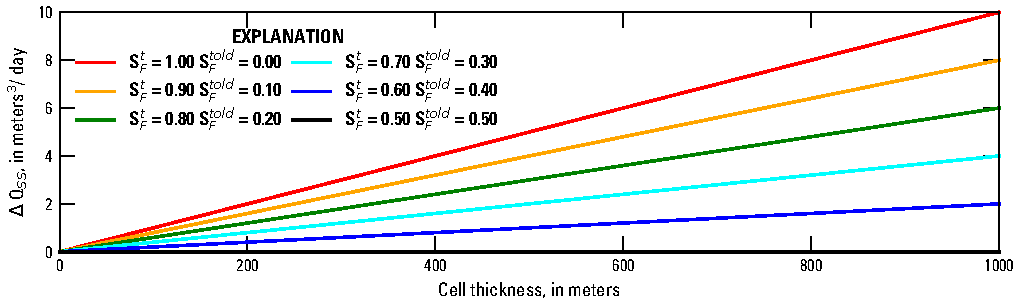
\includegraphics{./Figures/STOSsError.pdf}
	\caption[Graph showing changes in the flow from specific storage that result from changing the vertical datum]{Graph showing changes in the flow from specific storage, $Q_{SS}$, that result from changing the vertical datum from 0 to 1,000 m. The change in $Q_{SS}$ is plotted at a function of cell thickness, $\Delta z$, for various combinations of initial and final cell saturations, $S_F^\told$ and $S_F^t$. In this example, $\sps = 1\times10^{-5}$ m$^{-1}$, $A = 1$ m$^2$, and $\Delta t = 1$ d}
	\label{fig:orig-sserror}
	\end{center}
\end{figure}

A related deficiency of equation~\ref{eqn:STOeq-orig} concerns when a cell is dry either at the beginning ($S_F^\told = 0$) or the end ($S_F^t = 0$) of a time step, in which case the volumetric flow from specific storage equals 

\begin{align}
	\label{eqn:STOeq-def}
	Q_{SS} = \begin{dcases}
		\phantom{-} \frac{SC1}{\Delta t} S_F^\told h^\told & S_F^t = 0 \\
		- \frac{SC1}{\Delta t} S_F^t h^{t} & S_F^\told = 0
	\end{dcases} .
\end{align}

\noindent Equation~\ref{eqn:STOeq-def} can overestimate or underestimate the volumetric flow from specific storage, depending on the values of $h^\told$ and $h^t$, which in turn depend on the vertical datum. For example, in the case of a cell going dry ($S_F^\told > 0$, $S_F^t = 0$), water flows from specific storage, which implies $Q_{SS}$ is positive in sign. Because the cell is initially not dry, the initial cell head, $h^\told$, is above the cell bottom elevation. However, depending on the vertical datum, it is possible that $h^\told$ is negative in sign (with the cell bottom elevation being even more negative). In that case, equation~\ref{eqn:STOeq-def} calculates a negative value for $Q_{SS}$, which is opposite to what is expected on physical grounds.

\subsection{Revised Formulation}

To correct the deficiencies in the original specific storage formulation, the contribution of specific storage to the groundwater flow equation under water-table conditions is reexamined in terms of pressure head, which for a given elevation $z$ is defined as

\begin{equation}
	\label{eqn:pressure-head}
	\psi = h - z.
\end{equation}

\noindent The hydraulic head, $h$, associated with a MODFLOW cell is formally assigned to a point in the cell called the node, which under water-table conditions is at an elevation halfway between the cell bottom and the water table. The water-table elevation is, in turn, equal to the cell head, $h$. Thus, the value of the hydraulic head is the same at the node as it is at the water table, which is consistent with conceptualizing hydaulic head as being constant throughout the saturated portion of the cell. Extending this conceptualization to pressure head via equation~\ref{eqn:pressure-head} implies a linear variation of pressure head between a value of $0$ at the water table and a value of $h - BOT$ at the cell bottom. The revised specific storage formulation is therefore based on linear variation of pressure head with elevation within a cell.

The volumetric water content, $\theta$, at elevation $z$ within a cell is related to pressure head by

\begin{equation}
	\label{eqn:water_content}
	\begin{aligned}
		\theta = 
		\begin{dcases}
			\theta_r & z > h \\
			\sps \psi + S_y + \theta_r  & z \leq h
		\end{dcases},
	\end{aligned}
\end{equation}

\noindent where $\theta_r$ is the specific retention (unitless) and $S_y$ is the specific yield (unitless) in the cell. Integration of equation~\ref{eqn:water_content} from the bottom to the top of the cell gives the total volume of water stored in the cell:

\begin{equation}
	\label{eqn:storage-total-integrated}
	V_S = A \int_{BOT}^{TOP} \theta \, dz = A \int_{BOT}^{\zwts} \sps \psi \, dz + A \int_{BOT}^{\zwts} S_y \, dz + A \int_{BOT}^{TOP} \theta_r \, dz ,
\end{equation}

\noindent where $\zwts$ is the water-table elevation limited by the top elevation of the cell, given by

\begin{equation}
	\label{eqn:zwt}
	\zwts = BOT + \Delta z \, S_F .
\end{equation}

\noindent Assuming $\theta_r$, $S_y$, and $\sps$ are uniform throughout the cell, substitution of equation~\ref{eqn:pressure-head} into equation~\ref{eqn:storage-total-integrated} and evaluation of the integrals gives

\begin{equation}
	\label{eqn:storage-total}
	V_S = S_s A\ \Delta z\, S_F \left( h - \bar{z} \right) + S_y A\ \Delta z\, S_F + \theta_{r} A\ \Delta z ,
\end{equation}

\noindent where $\bar{z}$ is the node elevation (the vertical center of the saturated portion of the cell) given by

\begin{equation}
	\label{eqn:avg-z}
	\begin{aligned}
		\bar{z} = \frac{1}{\zwts - BOT} \int_{BOT}^{\zwts} z \, dz = BOT + \frac{\Delta z}{2} S_F .
	\end{aligned}
\end{equation}

The remainder of this chapter focuses on the contribution of specific storage (the first term on the right-hand side of equation~\ref{eqn:storage-total}) to the change in storage in a cell during a time step. The contribution of specific yield is calculated separately in \mf and remains unchanged by the revised approach described here. The volume of water in specific retention is assumed to be constant and therefore does not contribute to changes in storage.

Substitution of equations~\ref{eqn:STOeq-sc1} and~\ref{eqn:avg-z} into the first term on the right-hand side of equation~\ref{eqn:storage-total} gives the volume of water in compressible storage in the cell,

\begin{equation}
	\label{eqn:storage-ss-final}
	V_{SS} = SC1 \, S_F \left( h - BOT - \frac{\Delta z}{2} S_F \right) .
\end{equation}

\noindent The revised volumetric flow rate from compressible storage is then

\begin{equation}
	\label{eqn:STOeq-rev}
	Q_{SS} = \frac{SC1}{\Delta t} \left[ S_F^\told \left( h^\told - BOT - \frac{\Delta z}{2} S_F^\told \right) - S_F^t \left( h^t - BOT - \frac{\Delta z}{2} S_F^t \right) \right].
\end{equation}

\noindent When a cell is fully saturated ($S_F = 1$) at times $t$ and $\told$, equation~\ref{eqn:STOeq-rev} simplifies to

\begin{equation}
	\label{eqn:STOeq-rev-simp}
	Q_{SS} = \frac{SC1}{\Delta t} \left( h^\told - h^t \right) ,
\end{equation}

\noindent which is identical to the original specific storage formulation under confined conditions in \mf and the specific storage formulation under both confined and unconfined conditions in \mff \citep{modflow2005}.

The revised formulation in equation~\ref{eqn:STOeq-rev} is no longer dependent on the vertical datum because it involves cell saturations, $S_F$, and head differences of the form $h - BOT$, which do not change when the vertical datum changes. In the case of a cell being dry either at the beginning  or the end of a time step, the volumetric flow from specific storage based on the revised formulation equals 

\begin{align}
	\label{eqn:STOeq-def-rev}
	Q_{SS} = \begin{dcases}
		\phantom{-} \frac{SC1}{\Delta t} S_F^\told \left( h^\told - BOT - \frac{\Delta z}{2} S_F^\told \right) & S_F^t = 0 \\
		- \frac{SC1}{\Delta t} S_F^t \left( h^t - BOT - \frac{\Delta z}{2} S_F^t \right) & S_F^\told = 0
	\end{dcases} ,
\end{align}

\noindent which is the revised-formulation counterpart of equation~\ref{eqn:STOeq-def}. It can be deduced from equation~\ref{eqn:cell-saturation} that

\begin{equation}
	\label{eqn:hterm-sign}
	h - BOT - \frac{\Delta z}{2} S_F > 0 \quad \text{if \ $h > BOT$} ,
\end{equation}

\noindent which implies that equation~\ref{eqn:STOeq-def-rev} calculates the correct sign for $Q_{SS}$ when a cell goes dry or resaturates.

\subsection{Incorporation of the Revised Specific Storage Formulation into the CVFD Groundwater Flow Equation}

The approaches used to incorporate the contribution from specific storage into the linear matrix problem that represents the discretized groundwater flow equation are detailed below. When the standard formulation is used, the cell saturation defined in equation~\ref{eqn:cell-saturation} is used without modification. To allow for a smooth transition from dry (water level at or below the bottom of a cell) to fully saturated (water level at or above the top of the cell) conditions when the Newton formulation is used, quadratic smoothing is applied to the cell saturation over a small interval when the water level approaches the top or bottom of a cell, as described in in Eq.~4--5 in \cite{modflow6gwf}. 

\subsubsection{Standard Formulation}

Adding the cell number subscript ``$n$'' to cellwise quantities in equation~\ref{eqn:STOeq-rev} and adding specific storage terms dependent on the current value of head and known terms to the left- and right-hand sides of the discretized groundwater flow equation \citep[eq. 6--1]{modflow6gwf}, respectively, results in

\begin{equation}
	\label{eqn:STOeq-rev-fd}
	\begin{aligned}
		A_{n,n} \leftarrow & A_{n,n} - \frac{SC1_n}{\Delta t} S_{F_n}^\kmo \\
		b_n \leftarrow & b_n - \frac{SC1_n}{\Delta t} \biggl[ S_{F_n}^\told \left( h_n^\told - BOT_n - \frac{\Delta z_n}{2} S_{F_n}^\told \right) +  S_{F_n}^\kmo \left( BOT_n + \frac{\Delta z_n}{2} S_{F_n}^\kmo \right) \biggr],
	\end{aligned}
\end{equation} 

\noindent where $A_{n,n}$ is the diagonal of the coefficient matrix for cell $n$ and $b_n$ is the right-hand side of the groundwater flow equation for cell $n$. A variant of equation~\ref{eqn:STOeq-rev-fd} that tries to take advantage of the fact that

\begin{equation}
	\label{eqn:hterm-WTconditions}
	h_n - BOT_n - \frac{\Delta z_n}{2} S_{F_n} = \frac{1}{2} \left( h_n - BOT_n \right)
\end{equation}

\noindent under water-table conditions (head in the cell below the top of the cell) was also evaluated. However, the form presented in equation~\ref{eqn:STOeq-rev-fd} was found to converge better for the test problems evaluated and to simplify the additional terms added to the left- and right-hand sides of the discretized groundwater equation to complete the Newton-Raphson formulation.

\subsubsection{Newton-Raphson Formulation}

Adding the cell number subscript ``$n$'' to cellwise quantities in equation~\ref{eqn:STOeq-rev} and rearranging the equation to facilitate differentiation with respect to the current value of head, $h_n^t$, results in

\begin{equation}
	\label{eqn:STOeq-rev-2}
	Q_{SS_n} = \frac{SC1_n}{\Delta t} \left[S_{F_n}^\stold \left( h_n^\told - BOT_n - \frac{\Delta z_n}{2} S_{F_n}^\told \right) -S_{F_n}^\st \left( h_n^t - BOT_n \right) + \frac{\Delta z_n}{2} \left( S_{F_n}^\st \right)^2 \right] ,
\end{equation}

\noindent where $S_F^\ast$ is the quadratically smoothed cell saturation \citep[see][Eq.~4--5]{modflow6gwf}. The derivative of equation~\ref{eqn:STOeq-rev-2} with respect to $h_n$ is 

\begin{equation}
	\label{eqn:STOeq-rev-derv-simp}
	\frac{\partial Q_{SS_n}}{\partial h_n} = -\frac{SC1}{\Delta t} S_{F_n}^\skmo - \frac{SC1}{\Delta t} \frac{\partial S_{F_n}^\skmo}{\partial h_n} \left( h_n^\kmo - BOT_n \right) + \frac{SC1}{\Delta t} \Delta z_n S_{F_n}^\skmo  \frac{\partial S_{F_n}^\skmo}{\partial h_n} ,
\end{equation}

\noindent where the superscript ``$t$'' has been omitted for clarity, and the superscript ``$k-1$'' indicates quantities evaluated on the previous outer iteration of the solution procedure. The fully implicit form of the Newton-Raphson formulation for the contribution of specific storage in the cell in the form of equation 2--30 in \cite{modflow6gwf} is

\begin{equation}
	\label{eqn:STOeq-nr}
	\frac{\partial Q_{SS_n}}{\partial h_n} h_n^k = -Q_{SS_n} + \frac{\partial Q_{SS_n}}{\partial h_n} h_n^\kmo .
\end{equation}

\noindent Substitution of equations~\ref{eqn:STOeq-rev-2} and~\ref{eqn:STOeq-rev-derv-simp} into equation~\ref{eqn:STOeq-nr}  results in

\begin{equation}
	\label{eqn:STOeq-rev-nr-simp}
	\begin{split}
		A_{n,n} \leftarrow & A_{n,n} \biggl[ -\frac{SC1_n}{\Delta t}  S_{F_n}^\skmo - \frac{SC1}{\Delta t} \frac{\partial S_{F_n}^\kmo}{\partial h_n} \left( h_n^\kmo - BOT_n \right) + \frac{SC1}{\Delta t} \Delta z_n S_{F_n}^\kmo  \frac{\partial S_{F_n}^\skmo}{\partial h_n} \biggr]  \\
		b_n \leftarrow & b_n - \frac{SC1_n}{\Delta t} \biggl[ S_{F_n}^\stold \left( h_n^\told - BOT_n - \frac{\Delta z_n}{2} S_{F_n}^\stold \right) + S_{F_n}^\skmo \left( BOT_n + \frac{\Delta z_n}{2} S_{F_n}^\skmo \right) \biggr] \\
		& \phantom{b_n} + \biggl[ - \frac{SC1}{\Delta t} \frac{\partial S_{F_n}^\skmo}{\partial h_n} \left( h_n^\kmo - BOT_n \right) + \frac{SC1}{\Delta t} \Delta z_n S_{F_n}^\skmo  \frac{\partial S_{F_n}^\skmo}{\partial h_n} \biggr]  h_n^\kmo .
	\end{split}
\end{equation} 

\noindent Comparison of equation~\ref{eqn:STOeq-rev-nr-simp} to equation~\ref{eqn:STOeq-rev-fd} shows that many of the terms in the Newton-Raphson formulation were added as part of the standard formulation. The Newton-Raphson formulation is completed by adding the second and third terms on the right-hand side of equation~\ref{eqn:STOeq-rev-derv-simp} and the product of these terms and the current head to the terms already added to the diagonal of the coefficient matrix and right-hand side by the standard formulation, respectively.
